% ==============================================================================
% Relatório AutoML v2.0 - Equipe 9
% Universidade do Estado do Amazonas (UEA)
% Disciplina: Ciência de Dados
% Equipe 9: FLAML e LightAutoML
% ==============================================================================

\documentclass[11pt, a4paper, oneside]{article}

% ==============================================================================
% Encoding e idioma
% ==============================================================================
\usepackage[T1]{fontenc}
\usepackage[utf8]{inputenc}
\usepackage[brazil]{babel}

% ==============================================================================
% Layout
% ==============================================================================
\usepackage{geometry}
\usepackage{lmodern}
\usepackage{microtype}
\usepackage{setspace}
\usepackage{parskip}
\usepackage{fancyhdr}
\usepackage{lastpage}
\usepackage{titlesec}
\usepackage{tocloft}
\usepackage{float}
\usepackage{xurl}
\usepackage{amsmath}

% ==============================================================================
% Graficos, cores e diagramas
% ==============================================================================
\usepackage{graphicx}
\usepackage{xcolor}
\usepackage{tikz}

% ==============================================================================
% Tabelas e listas
% ==============================================================================
\usepackage{booktabs}
\usepackage{longtable}
\usepackage{tabularx}
\usepackage{array}
\usepackage{multirow}
\usepackage{colortbl}
\usepackage{ragged2e}
\usepackage{enumitem}

% ==============================================================================
% Caixas e codigo
% ==============================================================================
\usepackage{tcolorbox}
\tcbuselibrary{skins,breakable}
\usepackage{hyperref}

% ==============================================================================
% Geometria da pagina
% ==============================================================================
\geometry{
  a4paper,
  top=25mm, bottom=25mm,
  left=25mm, right=20mm,
  headheight=50mm, headsep=6mm,
  footskip=12mm
}

\graphicspath{{./}}
\setlength{\emergencystretch}{3em}
\setlength{\hfuzz}{2pt}
\setlength{\LTleft}{0pt}
\setlength{\LTright}{0pt}
\setlength{\tabcolsep}{4pt}
\Urlmuskip=0mu plus 2mu\relax

% ==============================================================================
% Cores (identidade UEA)
% ==============================================================================
\definecolor{ueagreen}{RGB}{26, 92, 42}
\definecolor{ueamint}{RGB}{74, 158, 107}
\definecolor{ueagray}{RGB}{88, 88, 90}
\definecolor{ueadark}{RGB}{30, 30, 30}
\definecolor{uealight}{RGB}{240, 248, 243}
\definecolor{tablehead}{RGB}{26, 92, 42}
\definecolor{tableheadlight}{RGB}{220, 240, 228}
\definecolor{tablealt}{RGB}{242, 250, 245}
\definecolor{alertcolor}{RGB}{180, 100, 0}
\definecolor{alertlight}{RGB}{255, 235, 210}
\definecolor{infolight}{RGB}{235, 248, 242}

% ==============================================================================
% Hyperref
% ==============================================================================
\hypersetup{
  colorlinks  = true,
  linkcolor   = ueagreen,
  urlcolor    = ueamint,
  citecolor   = ueagray,
  pdftitle    = {Relatório AutoML v2.0 - Equipe 9 - UEA Ciência de Dados},
  pdfauthor   = {Ana Beatriz Maciel Nunes, Fernando Luiz Da Silva Freire, Juliana Ballin Lima},
  pdfsubject  = {AutoML: FLAML e LightAutoML aplicados ao dataset ANP},
  pdfkeywords = {AutoML, FLAML, LightAutoML, ANP, Combustíveis, Ciência de Dados, UEA}
}

% ==============================================================================
% Tipos de coluna
% ==============================================================================
\newcolumntype{J}[1]{>{\justifying\arraybackslash\small}p{#1}}
\newcolumntype{L}[1]{>{\raggedright\arraybackslash\small}p{#1}}
\newcolumntype{C}[1]{>{\centering\arraybackslash\small}p{#1}}
\newcolumntype{Y}{>{\justifying\arraybackslash\small}X}
\renewcommand{\arraystretch}{1.25}

% ==============================================================================
% Formatacao de secoes
% ==============================================================================
\titleformat{\section}[block]
  {\Large\bfseries\color{ueagreen}}
  {\thesection}{1em}{}
  [\vspace{1pt}{\color{ueamint}\hrule height 1.5pt}\vspace{4pt}]

\titleformat{\subsection}[block]
  {\large\bfseries\color{ueagreen}}
  {\thesubsection}{1em}{}

\titleformat{\subsubsection}[block]
  {\normalsize\bfseries\color{ueagray}}
  {\thesubsubsection}{1em}{}

\titlespacing{\section}{0pt}{18pt}{6pt}
\titlespacing{\subsection}{0pt}{12pt}{4pt}
\titlespacing{\subsubsection}{0pt}{8pt}{2pt}

% ==============================================================================
% Helpers de logo
% ==============================================================================
\newcommand{\uealogo}{%
  \IfFileExists{uea-logo.png}{%
    \raisebox{-3mm}{%
      \begin{tikzpicture}
        \clip[rounded corners=1.4mm] (0,0) rectangle (27.65mm,14mm);
        \node[inner sep=0pt, anchor=south west] at (0,0)
          {
\includegraphics[height=14mm]{uea-logo.png}};
      \end{tikzpicture}%
    }%
  }{\textbf{\color{ueagreen}UEA}}%
}

\newcommand{\projlogo}{%
  \IfFileExists{../../diagrams/logo.png}{%
    
\includegraphics[height=12mm]{../../diagrams/logo.png}%
  }{\textcolor{ueagreen}{\small\textbf{ANP}}}%
}

% ==============================================================================
% Cabecalho e rodape
% ==============================================================================
\pagestyle{fancy}
\fancyhf{}
\fancyhead[L]{\uealogo}
\fancyhead[C]{\textcolor{ueagray}{\small Ciência de Dados $\cdot$ AutoML}}
\fancyhead[R]{\vspace{-2mm}\projlogo}
\fancyfoot[L]{\textcolor{ueagray}{\small UEA $\cdot$ Equipe 9}}
\fancyfoot[C]{\textcolor{ueagray}{\small\textbullet\quad\thepage\quad\textbullet}}
\fancyfoot[R]{\textcolor{ueagray}{\small v2.0}}
\renewcommand{\headrulewidth}{0.6pt}
\renewcommand{\headrule}{%
  \hbox to\headwidth{\color{ueagreen}\leaders\hrule height \headrulewidth\hfill}}
\renewcommand{\footrulewidth}{0.3pt}
\renewcommand{\footrule}{%
  \hbox to\headwidth{\color{ueagray}\leaders\hrule height \footrulewidth\hfill}}

% ==============================================================================
% Caixas utilitarias
% ==============================================================================
\newtcolorbox{notebox}{
  colback=alertlight,
  colframe=alertcolor,
  arc=2mm,
  boxrule=1.5pt,
  leftrule=4pt,
  sharp corners,
  breakable,
  enhanced
}

\newtcolorbox{infobox}{
  colback=infolight,
  colframe=ueamint,
  arc=2mm,
  boxrule=1.5pt,
  leftrule=4pt,
  sharp corners,
  breakable,
  enhanced
}

\newcommand{\thead}[1]{\cellcolor{tablehead}\color{white}\small\bfseries\shortstack[c]{#1}}
\newcommand{\taltrow}{\rowcolor{tablealt}}

% ==============================================================================
\begin{document}
% ==============================================================================

% ==============================================================================
% Capa
% ==============================================================================
\hypersetup{pageanchor=false}
\newgeometry{
  top=10mm, bottom=10mm,
  left=25mm, right=20mm,
  noheadfoot
}
\begin{titlepage}
  \thispagestyle{empty}
  \pagecolor{ueagreen}
  \color{white}
  \vspace*{\fill}

  \begin{center}
    \IfFileExists{uea-logo.png}{%
      \begin{tikzpicture}
        \clip[rounded corners=2.4mm] (0,0) rectangle (47.4mm,24mm);
        \node[inner sep=0pt, anchor=south west] at (0,0)
          {
\includegraphics[height=24mm]{uea-logo.png}};
      \end{tikzpicture}
    }{%
      {\fontsize{28}{34}\selectfont\textbf{UEA}}
    }\\[3mm]
    {\fontsize{15}{19}\selectfont Universidade do Estado do Amazonas}\\[1mm]
    {\fontsize{14}{18}\selectfont Escola Superior de Tecnologia}
  \end{center}

  \vspace{7mm}
  \noindent\textcolor{ueamint}{\rule{\textwidth}{1.5pt}}\\[4mm]
  {\fontsize{21}{26}\selectfont\textbf{Comparação de Ferramentas AutoML}}\\[3mm]
  {\fontsize{16}{21}\selectfont\textbf{FLAML e LightAutoML}}\\[3mm]
  {\fontsize{13}{17}\selectfont Aplicadas ao Dataset de Combustíveis ANP}\\[2mm]
  \noindent\textcolor{white}{\rule{\textwidth}{0.5pt}}

  \vspace{7mm}

  \begin{tabularx}{\textwidth}{@{}L{4cm} Y@{}}
    \textbf{Disciplina:}  & Ciência de Dados \\[2mm]
    \textbf{Equipe:}      & 9 \\[2mm]
    \textbf{Ferramentas:} & FLAML e LightAutoML \\[2mm]
    \textbf{Versão:}      & 2.0 \\[2mm]
    \textbf{Data:}        & 30 de maio de 2026 \\[2mm]
    \textbf{Integrantes:} & Ana Beatriz Maciel Nunes \\
                          & Fernando Luiz Da Silva Freire \\
                          & Juliana Ballin Lima \\
  \end{tabularx}

  \vspace{8mm}

  \begin{center}
    \IfFileExists{../../diagrams/logo.png}{%
      
\includegraphics[height=20mm]{../../diagrams/logo.png}
    }{}
  \end{center}

  \vspace{3mm}
  \noindent\textcolor{ueamint}{\rule{\textwidth}{0.5pt}}\\[2mm]
  \begin{center}
  \begin{minipage}{0.92\textwidth}
  \centering
  {\small Este relatório apresenta a Parte 1 (explicação teórica sobre AutoML), a
  Parte 2 (descrição do dataset utilizado) e a Parte 3 (aplicação prática da FLAML),
  agora ampliada com baseline, análise de erros e discussão de validade experimental,
  como segunda entrega da atividade de comparação de ferramentas AutoML da disciplina
  de Ciência de Dados na UEA.}
  \end{minipage}

  \vspace{3mm}
  {\small \textcopyright{} 2026 Equipe 9, Ciência de Dados, UEA. Uso acadêmico.}

  \vspace{2mm}
  {\small UEA $\cdot$ Equipe 9 $\bullet$ v2.0}
  \end{center}
  \vspace*{\fill}
\end{titlepage}
\restoregeometry
\hypersetup{pageanchor=true}
\setcounter{page}{1}

\pagecolor{white}
\color{ueadark}

% ==============================================================================
% Historico de versoes
% ==============================================================================
\thispagestyle{fancy}
\section*{Histórico de Versões}
\addcontentsline{toc}{section}{Histórico de Versões}

\begin{tabularx}{\textwidth}{@{}L{1.8cm} L{2.8cm} L{4cm} Y@{}}
  \toprule
  \thead{Versão} & \thead{Data} & \thead{Autores} & \thead{Descrição} \\
  \midrule
  1.0 & 26/05/2026 & Equipe 9 & Criação inicial do relatório. Parte 1: explicação teórica sobre AutoML. Parte 2: descrição do dataset ANP utilizado na atividade. \\
  \taltrow 2.0 & 26/05/2026 & Equipe 9 & Complemento da segunda entrega. Parte 3: aplicação da primeira ferramenta AutoML, FLAML, ao problema de regressão do preço médio da gasolina C. \\
  \taltrow 2.0 (rev.) & 30/05/2026 & Equipe 9 & Ampliação da Parte 3 com comparação a baselines simples, análise de erros por região e discussão de validade experimental. \\
  \bottomrule
\end{tabularx}

\vspace{6mm}

\begin{infobox}
\textbf{Organização dos relatórios da atividade:}
\begin{itemize}[leftmargin=1.2cm, topsep=2pt, itemsep=2pt]
  \item \textbf{v1.0}: Parte 1 - Explicação teórica sobre AutoML; Parte 2 - Descrição do dataset.
  \item \textbf{v2.0} (este documento): Parte 3 - Aplicação da FLAML, com baseline, análise de erros por região e discussão de validade experimental.
\end{itemize}
\end{infobox}

\newpage

% ==============================================================================
% Sumario
% ==============================================================================
\tableofcontents
\newpage

% ==============================================================================
% SECAO 1 - Explicacao Teorica sobre AutoML
% ==============================================================================
\section{Explicação Teórica sobre AutoML}
\label{sec:automl-teoria}

\begin{infobox}
Esta seção responde às questões teóricas solicitadas na atividade sobre AutoML, com
base nos slides disponibilizados na nota da disciplina
(\url{https://classroom.google.com/u/1/c/NzkzOTU2MDI1NjE4}) e com base em
pesquisa bibliográfica e compreensão conceitual da equipe.
\end{infobox}

% ------------------------------------------------------------------------------
\subsection{O que é AutoML?}
\label{sec:o-que-e-automl}
% ------------------------------------------------------------------------------

AutoML (Automated Machine Learning) é o conjunto de técnicas, ferramentas e processos
que automatizam etapas repetitivas e técnicas do ciclo de desenvolvimento de modelos
de Machine Learning. O objetivo central é reduzir o esforço manual necessário para
construir pipelines de ML de qualidade, desde a preparação dos dados até a seleção e
otimização do modelo final.

Diferentemente da abordagem tradicional, em que o cientista de dados realiza
manualmente cada escolha do pipeline, como a seleção do algoritmo, o ajuste de
hiperparâmetros e a engenharia de atributos, o AutoML executa essas etapas de forma
sistemática e automatizada. Isso é possível graças a técnicas como busca em espaço de
hiperparâmetros, otimização bayesiana, meta-aprendizado e avaliação cruzada automática.

O AutoML surgiu como resposta à crescente demanda por aplicações de ML em diferentes
domínios e à escassez de especialistas com domínio técnico profundo. Ferramentas como
FLAML, LightAutoML, AutoGluon, H2O AutoML e PyCaret representam implementações
práticas desse conceito, cada uma com diferentes abordagens e focos.

% ------------------------------------------------------------------------------
\subsection{Etapas de ML que podem ser automatizadas}
\label{sec:etapas-automatizadas}
% ------------------------------------------------------------------------------

Diversas etapas do ciclo de Machine Learning podem ser total ou parcialmente
automatizadas por ferramentas AutoML:

\begin{itemize}[leftmargin=1.5cm, itemsep=4pt]
  \item \textbf{Pré-processamento de dados:} imputação de valores ausentes, normalização e padronização de variáveis numéricas, codificação de variáveis categóricas (one-hot, label encoding) e detecção de tipos de dados.
  \item \textbf{Engenharia de atributos:} criação e transformação de features, seleção automática de atributos relevantes e redução de dimensionalidade.
  \item \textbf{Seleção de algoritmos:} comparação automática entre múltiplos algoritmos de ML (regressão linear, árvores de decisão, gradient boosting, redes neurais, entre outros).
  \item \textbf{Ajuste de hiperparâmetros:} busca automática das melhores configurações de cada modelo por meio de grid search, random search ou otimização bayesiana.
  \item \textbf{Avaliação e validação:} aplicação automática de validação cruzada (cross-validation), cálculo de métricas de desempenho e seleção do melhor modelo com base nos resultados.
  \item \textbf{Ensemble de modelos:} combinação automática de múltiplos modelos para melhorar o desempenho final (stacking, bagging, blending).
  \item \textbf{Geração de relatórios:} criação automática de resumos com métricas, importância de atributos e leaderboards comparativos.
\end{itemize}

% ------------------------------------------------------------------------------
\subsection{Etapas que ainda dependem da análise humana}
\label{sec:etapas-humanas}
% ------------------------------------------------------------------------------

Apesar do alto grau de automação, várias etapas do processo de ML ainda dependem
fundamentalmente da análise e julgamento humanos:

\begin{itemize}[leftmargin=1.5cm, itemsep=4pt]
  \item \textbf{Definição do problema:} identificar qual pergunta se quer responder, qual é a variável-alvo e que tipo de problema se trata (classificação, regressão, clustering).
  \item \textbf{Coleta e curadoria de dados:} obter, limpar e organizar os dados de forma adequada ao problema. A qualidade dos dados é responsabilidade humana.
  \item \textbf{Definição de métricas de avaliação:} escolher a métrica mais adequada ao contexto do negócio ou da pesquisa. Por exemplo, em problemas médicos, recall pode ser mais importante que precisão.
  \item \textbf{Interpretação dos resultados no contexto do domínio:} entender o significado prático das previsões do modelo e validar se fazem sentido no contexto real.
  \item \textbf{Avaliação ética e de vieses:} identificar e mitigar vieses presentes nos dados ou nos modelos, especialmente quando o modelo toma decisões que afetam pessoas.
  \item \textbf{Validação com especialistas do domínio:} verificar se os resultados são coerentes com o conhecimento especializado da área (saúde, finanças, engenharia, entre outras).
  \item \textbf{Implantação e monitoramento em produção:} decidir como integrar o modelo ao sistema real e como monitorar seu desempenho ao longo do tempo.
\end{itemize}

% ------------------------------------------------------------------------------
\subsection{Principais vantagens do AutoML}
\label{sec:vantagens}
% ------------------------------------------------------------------------------

O uso de ferramentas AutoML traz diversas vantagens práticas e estratégicas:

\begin{itemize}[leftmargin=1.5cm, itemsep=4pt]
  \item \textbf{Redução do tempo de desenvolvimento:} o processo que levaria dias ou semanas de experimentação manual pode ser realizado em horas.
  \item \textbf{Democratização do ML:} permite que analistas, pesquisadores e profissionais de outras áreas utilizem técnicas avançadas de ML sem precisar dominar todos os aspectos matemáticos e computacionais.
  \item \textbf{Exploração sistemática do espaço de modelos:} o AutoML explora combinações de algoritmos e hiperparâmetros de forma mais abrangente do que um humano poderia fazer manualmente.
  \item \textbf{Reprodutibilidade:} o processo automatizado garante que os experimentos possam ser replicados com os mesmos resultados.
  \item \textbf{Redução de erros humanos:} evita descuidos comuns na configuração manual de pipelines, como vazamento de dados (data leakage) e comparação inadequada de modelos.
  \item \textbf{Baseline rápido:} permite obter um modelo de referência (baseline) de qualidade rapidamente, antes de partir para ajustes manuais mais finos.
\end{itemize}

% ------------------------------------------------------------------------------
\subsection{Riscos e limitações do AutoML}
\label{sec:riscos}
% ------------------------------------------------------------------------------

O AutoML não é uma solução universal e apresenta riscos e limitações importantes que
devem ser considerados:

\begin{itemize}[leftmargin=1.5cm, itemsep=4pt]
  \item \textbf{Interpretabilidade reduzida:} os modelos gerados automaticamente, especialmente ensembles complexos, podem ser difíceis de interpretar e explicar para stakeholders não técnicos.
  \item \textbf{Alto custo computacional:} a busca automática por melhores modelos pode demandar muito tempo e recursos computacionais, especialmente em datasets grandes.
  \item \textbf{Risco de overfitting:} sem uma configuração adequada da validação, os modelos podem se ajustar excessivamente aos dados de treino e não generalizar bem.
  \item \textbf{Dependência da qualidade dos dados:} o AutoML não corrige problemas fundamentais nos dados de entrada. Um dataset com vieses ou erros produzirá modelos ruins independentemente da ferramenta utilizada.
  \item \textbf{Caixa-preta:} a automação pode obscurecer as escolhas feitas pelo sistema, dificultando o diagnóstico de problemas.
  \item \textbf{Limitações no domínio do problema:} nem sempre o AutoML encontra o melhor modelo para problemas muito específicos, que exigem conhecimento profundo do domínio para criar features relevantes.
\end{itemize}

% ------------------------------------------------------------------------------
\subsection{AutoML substitui o cientista de dados?}
\label{sec:substitui}
% ------------------------------------------------------------------------------

\textbf{Não.} O AutoML é uma ferramenta que potencializa o trabalho do cientista de
dados, mas não o substitui. As razões são diversas:

Em primeiro lugar, o AutoML automatiza tarefas técnicas e repetitivas, mas não é
capaz de definir o problema correto, compreender o contexto do negócio, avaliar a
qualidade e relevância dos dados nem interpretar os resultados à luz do conhecimento
especializado do domínio. Essas são competências essencialmente humanas.

Em segundo lugar, o uso irresponsável de AutoML sem compreensão do processo pode
levar a modelos tendenciosos, com vazamento de dados ou com métricas infladas que
não refletem o desempenho real. Somente um profissional com formação em Ciência de
Dados pode identificar e corrigir esses problemas.

Em terceiro lugar, a implantação de modelos em produção, o monitoramento de desvios
ao longo do tempo (concept drift) e as decisões éticas sobre uso de algoritmos em
contextos sensíveis exigem julgamento humano, responsabilidade e conhecimento
especializado que nenhuma ferramenta automatizada possui.

\begin{infobox}
\textbf{Conclusão:} AutoML é um acelerador poderoso no toolkit do cientista de dados.
Ele elimina parte do trabalho repetitivo, permite explorar mais alternativas em menos
tempo e facilita a construção de baselines rápidos. Mas o papel do cientista de dados
permanece insubstituível nas etapas que exigem julgamento, contexto e responsabilidade.
\end{infobox}

\newpage

% ==============================================================================
% SECAO 2 - Descricao do Dataset
% ==============================================================================
\section{Descrição do Dataset}
\label{sec:dataset}

% ------------------------------------------------------------------------------
\subsection{Identificação e Fonte}
\label{sec:dataset-fonte}
% ------------------------------------------------------------------------------

\begin{tabularx}{\textwidth}{@{}L{4.5cm} Y@{}}
  \toprule
  \textbf{Campo} & \textbf{Informação} \\
  \midrule
  \taltrow \textbf{Nome} & Dataset ANP - Análise de Preços e Volumes de Combustíveis (2021-2025) \\
  \textbf{Fonte} & Agência Nacional do Petróleo, Gás Natural e Biocombustíveis (ANP), bases públicas: Série Histórica do Levantamento de Preços e Vendas de Derivados de Petróleo e Biocombustíveis \\
  \taltrow \textbf{Disponibilidade} & Público, disponibilizado pela ANP no portal de dados abertos \\
  \textbf{Período} & Janeiro de 2021 a dezembro de 2025 \\
  \taltrow \textbf{Granularidade} & Mensal por Unidade Federativa (UF) \\
  \textbf{Arquivo processado} & \texttt{data/processed/dataset\_anp\_pca\_mds\_2021\_2025.csv} \\
  \bottomrule
\end{tabularx}

\vspace{6mm}

O dataset foi construído a partir do cruzamento entre duas bases públicas da ANP: a
série histórica de preços médios de revenda de combustíveis e os registros de volume
vendido (em m³) de derivados de petróleo e biocombustíveis. O merge foi realizado por
mês e sigla de UF, garantindo a inclusão de todas as 27 unidades federativas,
inclusive as da região Centro-Oeste, que apresentavam inconsistências nos nomes entre
as duas fontes originais.

% ------------------------------------------------------------------------------
\subsection{Estrutura dos Dados}
\label{sec:dataset-estrutura}
% ------------------------------------------------------------------------------

\begin{tabularx}{\textwidth}{@{}L{5.5cm} L{2.5cm} Y@{}}
  \toprule
  \thead{Atributo} & \thead{Tipo} & \thead{Descrição} \\
  \midrule
  \taltrow \texttt{mes\_ano} & Data & Mês e ano de referência da observação (formato YYYY-MM-01) \\
  \texttt{uf} & Categórico & Sigla da Unidade Federativa (ex.: AM, SP, RJ) \\
  \taltrow \texttt{uf\_nome} & Categórico & Nome completo da UF (ex.: AMAZONAS) \\
  \texttt{regiao} & Categórico & Região geográfica do Brasil (NORTE, NORDESTE, etc.) \\
  \taltrow \texttt{ano} & Numérico & Ano de referência (2021 a 2025) \\
  \texttt{mes} & Numérico & Mês de referência (1 a 12) \\
  \taltrow \texttt{preco\_medio\_gasolina\_c} & Numérico & Preço médio mensal de revenda da gasolina C (R\$/litro) \\
  \texttt{preco\_medio\_etanol\_hidratado} & Numérico & Preço médio mensal de revenda do etanol hidratado (R\$/litro) \\
  \taltrow \texttt{volume\_gasolina\_c\_m3} & Numérico & Volume vendido de gasolina C no mês (em m³) \\
  \texttt{volume\_etanol\_hidratado\_m3} & Numérico & Volume vendido de etanol hidratado no mês (em m³) \\
  \taltrow \texttt{volume\_total\_analisado\_m3} & Numérico & Soma dos volumes de gasolina C e etanol hidratado (em m³) \\
  \texttt{participacao\_etanol} & Numérico & Proporção do etanol no volume total analisado \\
  \taltrow \texttt{razao\_etanol\_gasolina} & Numérico & Razão entre volume de etanol e volume de gasolina C \\
  \texttt{preco\_relativo\_etanol\_gasolina} & Numérico & Razão entre preço do etanol e preço da gasolina C \\
  \taltrow \texttt{variacao\_preco\_gasolina\_c} & Numérico & Variação percentual mensal do preço da gasolina C \\
  \texttt{variacao\_volume\_gasolina\_c} & Numérico & Variação percentual mensal do volume vendido de gasolina C \\
  \bottomrule
\end{tabularx}

\vspace{4mm}

\begin{infobox}
\textbf{Dimensões do dataset:} 1.619 registros (observações UF-mês) e 16 atributos.
O dataset cobre os 27 estados brasileiros ao longo de 60 meses (jan/2021 a dez/2025),
resultando em uma cobertura praticamente completa do período analisado.
\end{infobox}

% ------------------------------------------------------------------------------
\subsection{Variável-Alvo}
\label{sec:dataset-target}
% ------------------------------------------------------------------------------

Para a atividade de AutoML, a variável-alvo escolhida é:

\begin{center}
  \begin{tcolorbox}[
    colback=tableheadlight,
    colframe=ueagreen,
    arc=2mm,
    boxrule=1.5pt,
    leftrule=4pt,
    width=0.85\textwidth,
    enhanced
  ]
    \centering
    \textbf{\large \texttt{preco\_medio\_gasolina\_c}}\\[2mm]
    \small Preço médio mensal de revenda da gasolina C, em R\$/litro,\\
    registrado por UF e mês de referência.
  \end{tcolorbox}
\end{center}

\vspace{4mm}

A variável \texttt{preco\_medio\_gasolina\_c} representa o preço médio de revenda da
gasolina C praticado em cada unidade federativa ao longo do tempo. Trata-se de uma
variável contínua, com valores que variam de aproximadamente R\$ 4,50 a R\$ 8,00
no período analisado, refletindo oscilações do mercado, variações regionais e efeitos
de políticas de combustíveis adotadas ao longo dos anos 2021 a 2025.

% ------------------------------------------------------------------------------
\subsection{Tipo de Problema}
\label{sec:dataset-tipo}
% ------------------------------------------------------------------------------

\textbf{Regressão.} O objetivo é prever o valor contínuo do preço médio da gasolina C
com base nos demais atributos disponíveis, como preço do etanol, volumes vendidos,
variações percentuais, participação do etanol no mercado, região geográfica e período
temporal. As ferramentas AutoML serão configuradas para este tipo de problema e
avaliadas pela métrica RMSE (Root Mean Squared Error) e pelo coeficiente de
determinação R².

% ------------------------------------------------------------------------------
\subsection{Justificativa para a Escolha do Dataset}
\label{sec:dataset-justificativa}
% ------------------------------------------------------------------------------

A equipe optou por utilizar o dataset já desenvolvido no projeto de Análise de
Combustíveis ANP com PCA e MDS pelos seguintes motivos:

\begin{enumerate}[leftmargin=1.5cm, itemsep=4pt]
  \item \textbf{Continuidade e integração:} o dataset está diretamente relacionado ao trabalho anterior da equipe nesta disciplina, permitindo uma análise mais rica e comparativa entre as técnicas não supervisionadas (PCA e MDS) e as técnicas supervisionadas via AutoML.
  \item \textbf{Relevância prática:} o preço dos combustíveis é um problema de interesse econômico real, com impacto direto no cotidiano da população e nas decisões de gestão de frotas, distribuição e políticas públicas.
  \item \textbf{Características adequadas para AutoML:} o dataset possui atributos numéricos e categóricos, tamanho moderado (1.619 registros), sem valores ausentes, e uma variável-alvo contínua bem definida, o que o torna adequado para um problema de regressão com AutoML.
  \item \textbf{Diversidade regional:} a presença de dados de todos os estados brasileiros e cinco regiões geográficas enriquece o problema de previsão com variações espaciais relevantes.
\end{enumerate}

% ------------------------------------------------------------------------------
\subsection{Qualidade dos Dados}
\label{sec:dataset-qualidade}
% ------------------------------------------------------------------------------

\begin{tabularx}{\textwidth}{@{}L{5.5cm} Y@{}}
  \toprule
  \thead{Aspecto} & \thead{Situação} \\
  \midrule
  \taltrow \textbf{Valores ausentes} & Nenhum. O dataset foi tratado antes da disponibilização, com remoção de registros incompletos e preenchimento via agregação mensal por UF. \\
  \textbf{Atributos categóricos} & Presentes: \texttt{uf} (27 categorias), \texttt{uf\_nome} (27 categorias), \texttt{regiao} (5 categorias). As ferramentas AutoML realizarão a codificação automaticamente. \\
  \taltrow \textbf{Dados desbalanceados} & Não aplicável ao problema de regressão. Todos os estados têm distribuição temporal aproximadamente uniforme (60 meses cada). \\
  \textbf{Escala das variáveis} & As variáveis numéricas possuem escalas distintas (preços em R\$/litro, volumes em m³, proporções de 0 a 1). A padronização será realizada automaticamente pelas ferramentas AutoML. \\
  \taltrow \textbf{Outliers} & São Paulo apresenta volumes de vendas significativamente maiores que os demais estados, caracterizando um outlier por escala. Essa característica já foi identificada na análise exploratória com PCA realizada anteriormente pela equipe. \\
  \textbf{Período temporal} & O dataset cobre jan/2021 a dez/2025. A variável temporal (\texttt{mes\_ano}) é tratada como atributo numérico (ano e mês separados) para compatibilidade com os algoritmos AutoML. \\
  \bottomrule
\end{tabularx}

\vspace{6mm}

\begin{notebox}
\textbf{Divisão treino e teste:} para manter comparabilidade entre as ferramentas
AutoML (FLAML e LightAutoML), será utilizada a mesma divisão para ambas: 80\% dos
registros para treino e 20\% para teste, com seleção aleatória estratificada por
região geográfica. A mesma semente aleatória (random state = 42) será aplicada em
ambas as ferramentas.
\end{notebox}

% ==============================================================================
% SECAO 3 - Aplicacao da Primeira Ferramenta AutoML
% ==============================================================================
\newpage
\section{Aplicação da Primeira Ferramenta AutoML}
\label{sec:flaml}

% ------------------------------------------------------------------------------
\subsection{Nome e breve descrição da ferramenta}
\label{sec:flaml-descricao}
% ------------------------------------------------------------------------------

A primeira ferramenta aplicada foi a \textbf{FLAML} (Fast and Lightweight AutoML),
uma biblioteca voltada à busca eficiente de bons modelos com baixo custo
computacional. Seu diferencial está em explorar, de forma automática, candidatos de
modelos e combinações de hiperparâmetros dentro de um orçamento de tempo definido,
priorizando eficiência sem abrir mão de desempenho competitivo.

Neste experimento, a FLAML foi utilizada em uma tarefa de \textbf{regressão tabular},
com o objetivo de prever a variável \texttt{preco\_medio\_gasolina\_c}. O problema é
adequado a uma ferramenta AutoML porque envolve dados estruturados, mistura de
atributos numéricos e categóricos, e relações potencialmente não lineares entre preço,
volume, região e tempo.

\begin{infobox}
\textbf{Objetivo da Parte 3:} aplicar a primeira ferramenta AutoML atribuída à equipe,
documentar o fluxo experimental, apresentar os modelos avaliados automaticamente,
analisar o melhor resultado obtido e discutir, de forma crítica, os limites da
aplicação.
\end{infobox}

% ------------------------------------------------------------------------------
\subsection{Instalação e acesso}
\label{sec:flaml-instalacao}
% ------------------------------------------------------------------------------

A execução foi realizada em ambiente virtual Python local, no próprio projeto. As
dependências necessárias foram registradas em \texttt{requirements.txt}, incluindo
\texttt{flaml} e \texttt{lightgbm}, de modo a permitir reprodução do experimento em
outro ambiente compatível.

\begin{tabularx}{\textwidth}{@{}L{4.8cm} Y@{}}
  \toprule
  \thead{Etapa} & \thead{Comando utilizado} \\
  \midrule
  \taltrow Criar ambiente virtual & \texttt{python -m venv .venv} \\
  Ativar ambiente & \texttt{source .venv/bin/activate} \\
  \taltrow Instalar dependências & \texttt{pip install -r requirements.txt} \\
  Executar experimento FLAML & \texttt{python -m src.flaml\_analysis} \\
  \bottomrule
\end{tabularx}

\vspace{4mm}

O script reprodutível do experimento foi implementado em
\texttt{src/flaml\_analysis.py}. Ele carrega o dataset processado, aplica a mesma
divisão treino e teste definida na Parte 2, treina a FLAML, registra as métricas e
gera os gráficos de apoio utilizados na análise.

% ------------------------------------------------------------------------------
\subsection{Preparação para o experimento}
\label{sec:flaml-preparacao}
% ------------------------------------------------------------------------------

O arquivo utilizado foi
\texttt{data/processed/dataset\_anp\_pca\_mds\_2021\_2025.csv}, com 1.619 registros.
A divisão usada foi de 80\% para treino e 20\% para teste, com
\texttt{random\_state = 42}. Isso gerou 1.295 registros de treino e 324 registros de
teste.

Para evitar vazamento de dados e manter a avaliação o mais honesta possível, algumas
colunas foram removidas da modelagem supervisionada:

\begin{itemize}[leftmargin=1.5cm, itemsep=4pt]
  \item \texttt{preco\_medio\_gasolina\_c}: variável-alvo.
  \item \texttt{variacao\_preco\_gasolina\_c}: variável derivada diretamente do preço da gasolina C, o que poderia facilitar artificialmente a previsão.
  \item \texttt{preco\_relativo\_etanol\_gasolina}: razão que usa o preço da gasolina C no denominador, criando dependência direta com o alvo.
  \item \texttt{mes\_ano}: substituída por \texttt{ano} e \texttt{mes} para facilitar o tratamento numérico pelas ferramentas AutoML.
  \item \texttt{uf\_nome}: removida por duplicar a informação já contida em \texttt{uf}.
\end{itemize}

As colunas categóricas \texttt{uf} e \texttt{regiao} foram codificadas por
\textit{one-hot encoding}. Após essa transformação, a matriz de modelagem passou de
11 atributos originais para 41 atributos numéricos.

\begin{tabularx}{\textwidth}{@{}L{5.2cm} Y@{}}
  \toprule
  \thead{Configuração} & \thead{Valor} \\
  \midrule
  \taltrow Tipo de problema & Regressão \\
  Variável-alvo & \texttt{preco\_medio\_gasolina\_c} \\
  \taltrow Métrica principal & RMSE \\
  Divisão dos dados & 80\% treino e 20\% teste \\
  \taltrow Estratificação & Aplicada por região geográfica (\texttt{regiao}) \\
  Semente aleatória & 42 \\
  \taltrow Orçamento de tempo & 60 segundos \\
  Estimadores avaliados & \texttt{lgbm}, \texttt{rf}, \texttt{extra\_tree} \\
  \bottomrule
\end{tabularx}

\vspace{4mm}

A escolha por uma configuração enxuta foi intencional: a proposta desta etapa era
avaliar a capacidade da FLAML de construir um bom baseline em pouco tempo, sem recorrer
a um processo manual extenso de tuning.

\begin{infobox}
\textbf{Sobre a estratificação:} embora a tarefa seja de regressão, a estratificação
foi aplicada sobre a variável categórica \texttt{regiao}, e não sobre a variável-alvo
numérica. Essa decisão preserva a proporção das cinco regiões geográficas entre treino
e teste, evitando concentração regional por efeito do sorteio aleatório. Isso é coerente
com o planejamento descrito na Parte 2 deste relatório.
\end{infobox}

% ------------------------------------------------------------------------------
\subsection{Principais comandos e etapas utilizadas}
\label{sec:flaml-etapas}
% ------------------------------------------------------------------------------

As principais etapas executadas no script foram:

\begin{enumerate}[leftmargin=1.5cm, itemsep=4pt]
  \item Carregamento do dataset processado da ANP.
  \item Separação da variável-alvo \texttt{preco\_medio\_gasolina\_c}.
  \item Remoção de colunas que poderiam causar vazamento de dados.
  \item Codificação das variáveis categóricas \texttt{uf} e \texttt{regiao}.
  \item Divisão treino e teste com 20\% dos registros no conjunto de teste.
  \item Configuração da FLAML para regressão, métrica RMSE e orçamento de 60 segundos.
  \item Treinamento automático dos modelos candidatos.
  \item Avaliação do melhor modelo no conjunto de teste.
  \item Geração de métricas, \textit{leaderboard}, previsões e gráficos.
\end{enumerate}

% ------------------------------------------------------------------------------
\subsection{Modelos testados automaticamente}
\label{sec:flaml-modelos}
% ------------------------------------------------------------------------------

A FLAML avaliou três famílias de modelos dentro do orçamento definido. O melhor
resultado de validação interna foi obtido pelo estimador \texttt{lgbm}, baseado em
LightGBM, que conseguiu equilibrar erro baixo e uso eficiente do tempo disponível.

\begin{tabularx}{\textwidth}{@{}L{3cm} C{4cm} C{3cm} Y@{}}
  \toprule
  \thead{Estimador} & \thead{RMSE de validação} & \thead{Selecionado} & \thead{Observação} \\
  \midrule
  \taltrow \texttt{lgbm} & 0,1255 & Sim & Melhor equilíbrio entre erro e tempo dentro do orçamento definido. \\
  \texttt{extra\_tree} & 0,1287 & Não & Resultado próximo ao melhor modelo, com desempenho competitivo. \\
  \taltrow \texttt{rf} & 0,2501 & Não & Desempenho inferior no orçamento de tempo disponível. \\
  \bottomrule
\end{tabularx}

\vspace{4mm}

A melhor configuração encontrada para o \texttt{lgbm} utilizou, entre outros
hiperparâmetros, \texttt{n\_estimators = 1294}, \texttt{num\_leaves = 22},
\texttt{learning\_rate = 0,0132}, \texttt{min\_child\_samples = 9} e
\texttt{colsample\_bytree = 0,5934}. Esses valores indicam um modelo relativamente
flexível, mas ainda controlado o suficiente para reduzir risco de overfitting.

% ------------------------------------------------------------------------------
\subsection{Melhor modelo e métricas obtidas}
\label{sec:flaml-resultados}
% ------------------------------------------------------------------------------

O melhor modelo final encontrado pela FLAML foi um \textbf{LightGBM Regressor}
(\texttt{lgbm}). A avaliação abaixo foi calculada no conjunto de teste, que não foi
utilizado para treinamento.

\begin{center}
\begin{tabularx}{0.9\textwidth}{@{}L{4.5cm} C{4cm} Y@{}}
  \toprule
  \thead{Métrica} & \thead{Valor} & \thead{Interpretação} \\
  \midrule
  \taltrow RMSE & 0,1148 & Erro médio quadrático em R\$/litro, com penalização maior para erros elevados. \\
  MAE & 0,0819 & Erro absoluto médio aproximado de oito centavos por litro. \\
  \taltrow R² & 0,9693 & O modelo explicou cerca de 96,93\% da variação observada no teste. \\
  MAPE & 1,3841\% & Erro percentual médio baixo para o recorte testado. \\
  \bottomrule
\end{tabularx}
\end{center}

\vspace{3mm}

O tempo aproximado de execução foi de \textbf{60,78 segundos}. Em termos práticos,
isso mostra que a FLAML conseguiu produzir um modelo competitivo em pouco tempo, com
intervenção manual mínima da equipe.

\begin{figure}[H]
  \centering
  \IfFileExists{flaml_real_vs_previsto.png}{%
    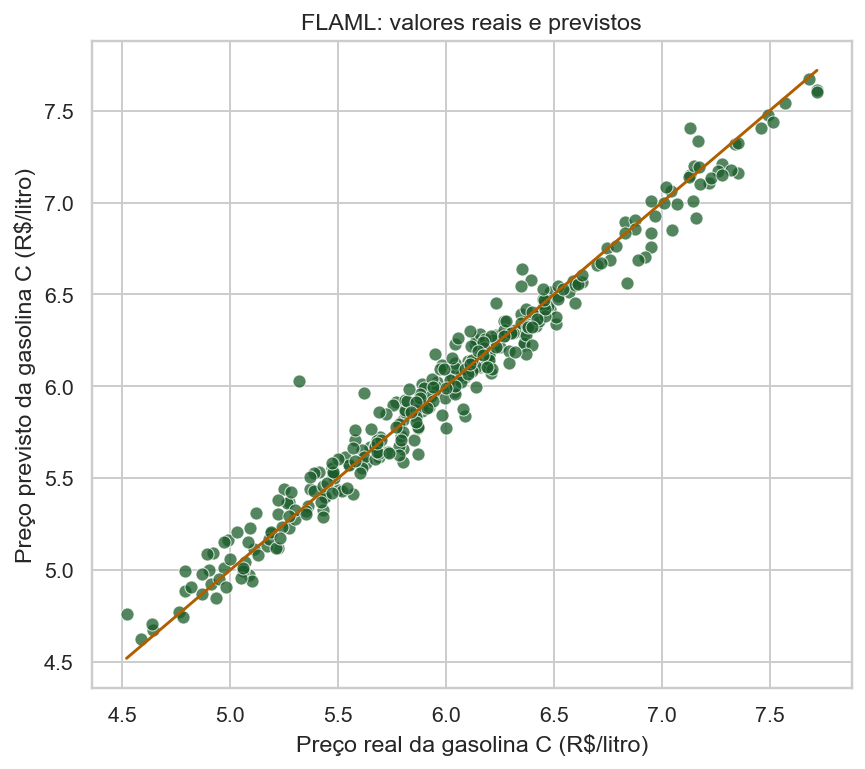
\includegraphics[width=0.78\textwidth]{flaml_real_vs_previsto.png}
  }{%
    % figura disponível
  }
  \caption{Comparação entre os valores reais e previstos pela FLAML no conjunto de teste.}
  \label{fig:flaml-real-previsto}
\end{figure}

\begin{infobox}
\textbf{Leitura dos resultados:} o valor de RMSE ficou baixo na escala do problema,
enquanto o R² elevado indica que a maior parte da variação do preço da gasolina C foi
capturada pelo modelo. Ainda assim, trata-se de um resultado preditivo em dados
históricos, e não de uma demonstração de causalidade.
\end{infobox}

% ------------------------------------------------------------------------------
\subsection{Recursos gerados pela ferramenta}
\label{sec:flaml-recursos}
% ------------------------------------------------------------------------------

O experimento gerou os seguintes artefatos no projeto:

\begin{tabularx}{\textwidth}{@{}L{6.2cm} Y@{}}
  \toprule
  \thead{Arquivo} & \thead{Conteúdo} \\
  \midrule
  \taltrow \path{outputs/tables/flaml_metricas.csv} & Métricas finais no conjunto de teste, melhor estimador, tempo de execução e configuração geral. \\
  \path{outputs/tables/flaml_leaderboard.csv} & Comparação dos estimadores avaliados automaticamente pela FLAML. \\
  \taltrow \path{outputs/tables/flaml_importancia_atributos.csv} & Importância dos atributos do melhor modelo final. \\
  \path{outputs/tables/flaml_previsoes_teste.csv} & Valores reais, previsões e erros no conjunto de teste. \\
  \taltrow \path{outputs/tables/flaml_configuracao.json} & Configuração final do melhor modelo e parâmetros do experimento. \\
  \path{outputs/tables/flaml_baseline_comparacao.csv} & Comparação do desempenho da FLAML com baselines simples. \\
  \taltrow \path{outputs/tables/flaml_analise_erros_regiao.csv} & Resumo dos erros médios por região no conjunto de teste. \\
  \path{outputs/tables/flaml_resumo_erros.csv} & Estatísticas resumidas da distribuição dos resíduos. \\
  \taltrow \path{outputs/tables/flaml_top_importancias.csv} & Ranking das principais variáveis do modelo. \\
  \path{outputs/figures/flaml_real_vs_previsto.png} & Gráfico de valores reais contra valores previstos. \\
  \taltrow \path{outputs/figures/flaml_importancia_atributos.png} & Gráfico dos principais atributos do melhor modelo. \\
  \path{outputs/figures/flaml_baseline_rmse.png} & Comparação visual do RMSE com baselines. \\
  \taltrow \path{outputs/figures/flaml_mae_por_regiao.png} & Erro absoluto médio por região. \\
  \path{outputs/figures/flaml_hist_erro_absoluto.png} & Distribuição dos erros absolutos. \\
  \bottomrule
\end{tabularx}

\vspace{4mm}

Entre os atributos mais importantes para o melhor modelo, destacaram-se o preço médio
do etanol hidratado, a participação do etanol, o volume de etanol hidratado, a
variação de volume da gasolina C e o volume de gasolina C. A leitura é coerente com o
contexto do problema: preços e volumes dos combustíveis se relacionam por dinâmica de
mercado, competição entre combustíveis e diferenças regionais de consumo.

\begin{figure}[H]
  \centering
  \IfFileExists{flaml_importancia_atributos.png}{%
    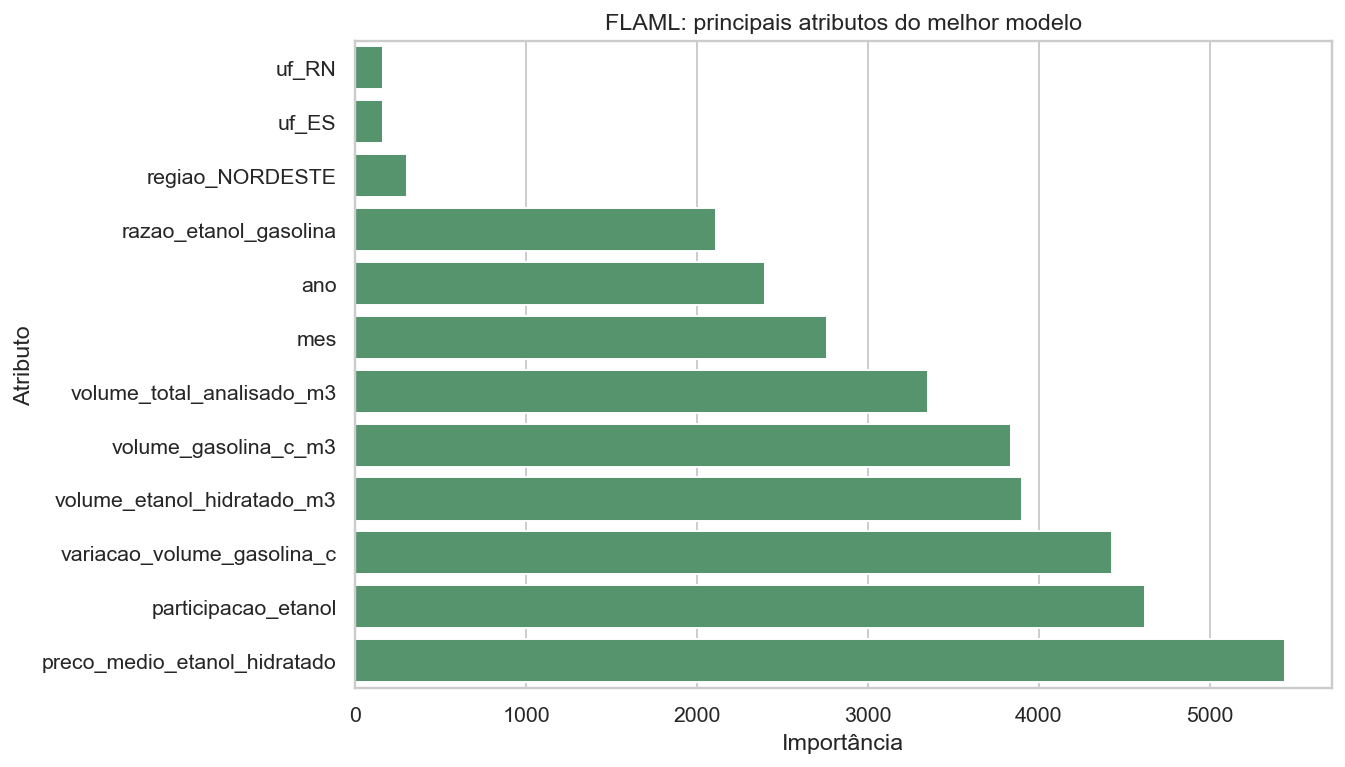
\includegraphics[width=0.86\textwidth]{flaml_importancia_atributos.png}
  }{%
    % figura disponível
  }
  \caption{Principais atributos do melhor modelo selecionado pela FLAML.}
  \label{fig:flaml-importancia}
\end{figure}


% ------------------------------------------------------------------------------
\subsection{Comparação com baselines simples}
\label{sec:flaml-baselines}

Para avaliar o quanto a FLAML realmente agregou valor ao problema, a equipe comparou o
resultado obtido com baselines simples construídos a partir do próprio conjunto de
treinamento. Essa comparação é importante porque métricas altas, isoladamente, nem
sempre indicam que o modelo superou estratégias ingênuas de previsão.

\begin{table}[H]
\centering
\small
\setlength{\tabcolsep}{4.2pt}
\begin{tabularx}{\textwidth}{@{}Y C{1.45cm} C{1.45cm} C{1.25cm} C{1.45cm} C{1.8cm}@{}}
  \toprule
  \thead{Modelo} & \thead{RMSE} & \thead{MAE} & \thead{R²} & \thead{MAPE} & \thead{Melhora\\RMSE} \\
  \midrule
  \taltrow FLAML (\texttt{lgbm}) & 0,1148 & 0,0819 & 0,9693 & 1,3841\% & 82,5\% \\
  Média do treino & 0,6553 & 0,5165 & \textasciitilde 0,0000 & 8,7384\% & -- \\
  \taltrow Média por região & 0,6467 & 0,5112 & 0,0262 & 8,6633\% & -- \\
  Média por UF & 0,6291 & 0,4921 & 0,0785 & 8,3699\% & -- \\
  \bottomrule
\end{tabularx}
\caption{Comparação entre a FLAML e baselines simples calculados a partir do conjunto de treino.}
\label{tab:flaml-baselines}
\end{table}

A comparação mostra que o modelo selecionado pela FLAML superou com folga os
baselines ingênuos. Em relação à predição pela média do treino, o RMSE caiu de 0,6553
para 0,1148, uma redução de aproximadamente 82,5\%. Mesmo o baseline mais informativo,
baseado na média por UF, permaneceu muito acima do erro obtido pela FLAML.

Esse resultado indica que a ferramenta foi capaz de explorar relações não lineares e
interações entre variáveis que os baselines não capturam. Na prática, isso reforça que
o experimento não apenas produziu um modelo com bom desempenho absoluto, mas também
gerou valor real em comparação com estratégias extremamente simples.

\begin{figure}[H]
  \centering
  \IfFileExists{flaml_baseline_rmse.png}{%
    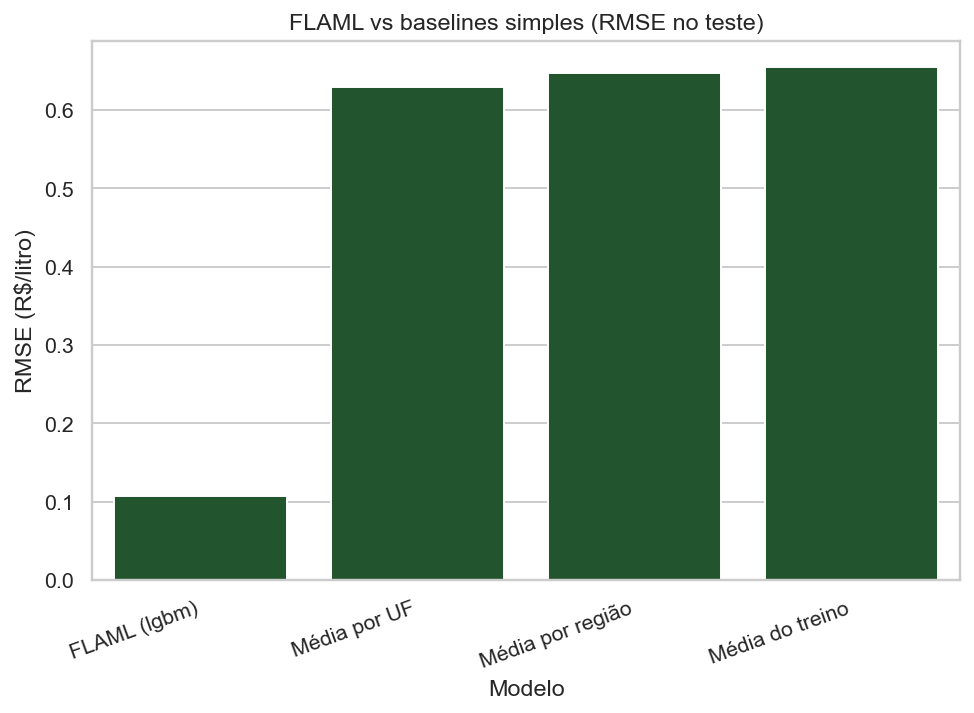
\includegraphics[width=0.78\textwidth]{flaml_baseline_rmse.png}
  }{%
    \begin{infobox}Os dados desta comparação estão disponíveis na Tabela~\ref{tab:flaml-baselines}.\end{infobox}
  }
  \caption{Comparação do RMSE da FLAML com baselines simples.}
  \label{fig:flaml-baseline-rmse}
\end{figure}

% ------------------------------------------------------------------------------
\subsection{Análise dos erros no conjunto de teste}
\label{sec:flaml-erros}

Além das métricas globais, a análise dos resíduos ajuda a entender onde o modelo se
comporta melhor e onde ele encontra mais dificuldade. No conjunto de teste, o erro
absoluto médio foi de 0,0819, com mediana de 0,0586. Metade das previsões teve erro
absoluto abaixo de 0,0586, e 95\% ficaram abaixo de 0,2164.

\begin{table}[H]
\centering
\small
\setlength{\tabcolsep}{5pt}
\begin{tabularx}{0.78\textwidth}{@{}Y C{2.35cm}@{}}
  \toprule
  \thead{Resumo do erro} & \thead{Valor} \\
  \midrule
  \taltrow Mediana do erro absoluto & 0,0586 \\
  75\% dos erros absolutos & 0,1155 \\
  \taltrow 90\% dos erros absolutos & 0,1843 \\
  95\% dos erros absolutos & 0,2164 \\
  Máximo erro absoluto & 0,7992 \\
  \taltrow Desvio-padrão do erro assinado & 0,1150 \\
  Erro médio assinado & -0,0002 \\
  \bottomrule
\end{tabularx}
\caption{Resumo da distribuição dos resíduos da FLAML no conjunto de teste.}
\label{tab:flaml-resumo-erros}
\end{table}

A distribuição dos erros mostra que a maior parte das previsões ficou próxima do valor
real, sem viés sistemático relevante, já que o erro médio assinado ficou praticamente
nulo. O maior erro absoluto observado foi concentrado em um caso específico da região
Norte, o que sugere sensibilidade maior em alguns pontos com menor representatividade
no conjunto de teste.

\begin{table}[H]
\centering
\small
\setlength{\tabcolsep}{4.5pt}
\begin{tabularx}{0.92\textwidth}{@{}Y C{1.45cm} C{1.45cm} C{1.6cm} C{1.6cm}@{}}
  \toprule
  \thead{Região} & \thead{MAE} & \thead{RMSE} & \thead{Erro médio} & \thead{MAPE} \\
  \midrule
  \taltrow CENTRO OESTE & 0,0687 & 0,0951 & 0,0099 & 1,1804\% \\
  SUDESTE & 0,0702 & 0,1062 & -0,0076 & 1,2052\% \\
  \taltrow NORDESTE & 0,0802 & 0,1004 & 0,0128 & 1,3293\% \\
  NORTE & 0,0902 & 0,1409 & -0,0055 & 1,5240\% \\
  \taltrow SUL & 0,1011 & 0,1227 & -0,0308 & 1,7318\% \\
  \bottomrule
\end{tabularx}
\caption{Erro médio da FLAML por região no conjunto de teste.}
\label{tab:flaml-erro-regiao}
\end{table}

Em nível regional, o Centro-Oeste e o Sudeste tiveram os menores erros médios, enquanto
o Sul apresentou o maior MAE entre as cinco regiões. Ainda assim, a diferença entre as
regiões não foi dramática, e todos os valores permaneceram em patamares baixos para um
problema de regressão tabular. Isso indica que o modelo aprendeu padrões relativamente
estáveis, mas ainda há espaço para refinamento em regiões com maior heterogeneidade.

\begin{figure}[H]
  \centering
  \IfFileExists{flaml_mae_por_regiao.png}{%
    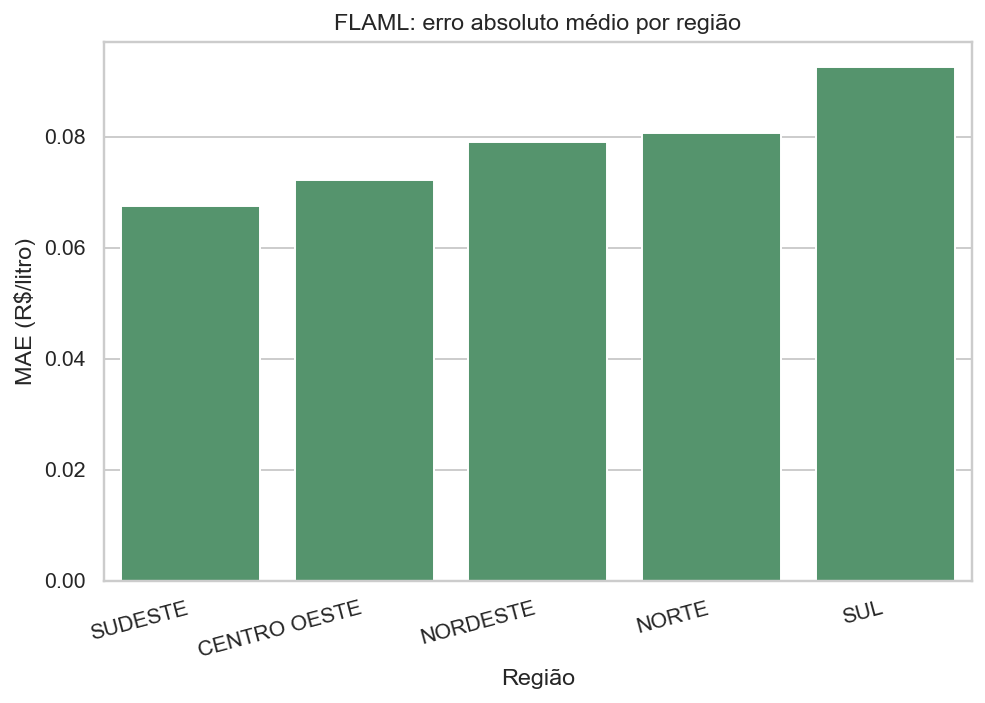
\includegraphics[width=0.78\textwidth]{flaml_mae_por_regiao.png}
  }{%
    \begin{infobox}Os dados estão disponíveis na Tabela~\ref{tab:flaml-erro-regiao}.\end{infobox}
  }
  \caption{Erro absoluto médio da FLAML por região.}
  \label{fig:flaml-mae-regiao}
\end{figure}

\begin{figure}[H]
  \centering
  \IfFileExists{flaml_hist_erro_absoluto.png}{%
    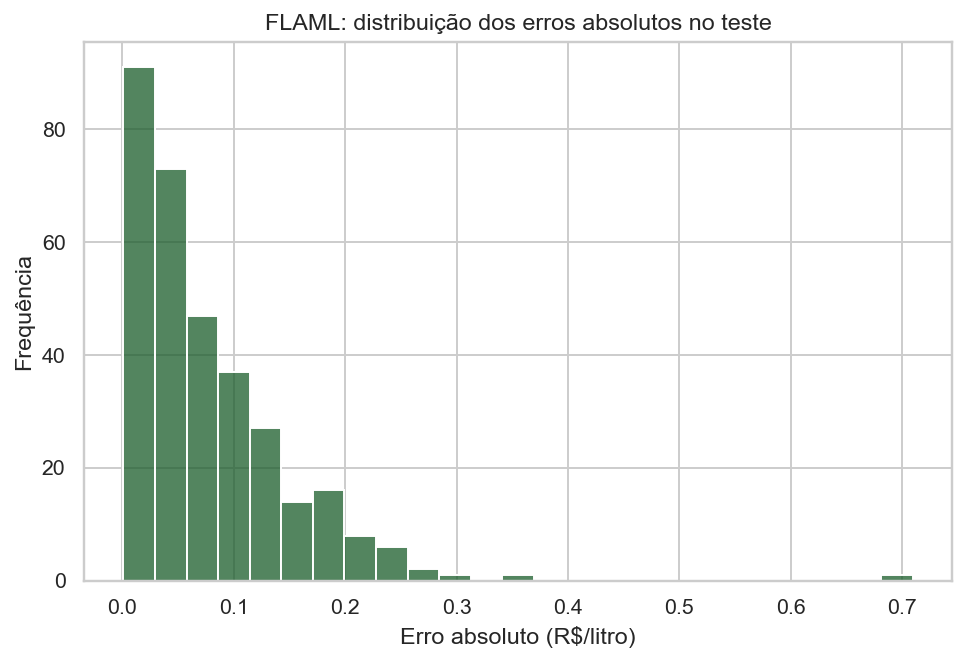
\includegraphics[width=0.78\textwidth]{flaml_hist_erro_absoluto.png}
  }{%
    \begin{infobox}Os dados estão disponíveis na Tabela~\ref{tab:flaml-resumo-erros}.\end{infobox}
  }
  \caption{Distribuição dos erros absolutos da FLAML no conjunto de teste.}
  \label{fig:flaml-hist-erro}
\end{figure}

% ------------------------------------------------------------------------------
\subsection{Validade experimental e ameaças à generalização}
\label{sec:flaml-validade}

Os resultados obtidos demonstram que a FLAML foi capaz de construir um modelo com
elevado desempenho preditivo para o conjunto de dados analisado. Entretanto, algumas
limitações metodológicas devem ser consideradas ao interpretar esses números.

Em primeiro lugar, o experimento foi conduzido com dados históricos de 2021 a 2025.
Dessa forma, o modelo aprende padrões presentes nesse intervalo temporal específico e
não há garantia de que o mesmo desempenho será mantido em cenários futuros sujeitos a
mudanças econômicas, tributárias ou regulatórias.

Além disso, apesar de as colunas que poderiam causar vazamento direto terem sido
removidas, ainda existem atributos fortemente correlacionados com a variável-alvo. Isso
ajuda a explicar o alto desempenho observado, mas também significa que o modelo está
aprendendo relações estatísticas muito informativas do próprio contexto de mercado.

Outro ponto importante é que esta etapa não teve como objetivo construir um sistema
operacional de previsão em produção. O foco foi avaliar a capacidade da ferramenta
AutoML de encontrar automaticamente modelos competitivos em um problema tabular de
regressão.

Por fim, métricas elevadas não implicam causalidade. O modelo identifica padrões
associativos presentes nos dados, mas não determina relações de causa e efeito entre
preços, volumes de venda, região geográfica e período temporal.
% ------------------------------------------------------------------------------
\subsection{Interpretação e fechamento da primeira aplicação}
\label{sec:flaml-interpretacao}

A FLAML apresentou desempenho muito forte na tarefa de regressão, com RMSE de 0,1148
no conjunto de teste e R² de 0,9693. Em termos práticos, o modelo consegue reproduzir
com boa precisão a estrutura dos preços observados no período analisado, mantendo erro
absoluto médio inferior a nove centavos por litro.

O ganho em relação aos baselines simples confirma que o bom desempenho não veio apenas
da estabilidade média dos dados. Mesmo quando comparado ao baseline por UF, que já é
mais informativo do que a média global, a FLAML permaneceu substancialmente melhor.
Isso sugere que a ferramenta conseguiu capturar interações entre variáveis de mercado,
região e período que são úteis para a tarefa.

Ao mesmo tempo, a interpretação deve continuar sendo cautelosa. O modelo aprendeu
padrões históricos e não estabelece causalidade entre as variáveis. Além disso, o
experimento usa dados do mesmo período da observação, o que favorece a modelagem
supervisionada, mas não equivale automaticamente a um cenário de previsão futura em
produção.

A análise feita nesta etapa cumpre, portanto, um papel metodológico claro: mostrar que
a FLAML é uma opção eficiente para obter um baseline forte em pouco tempo, com boa
capacidade preditiva e baixa intervenção manual. Isso prepara o terreno para a
comparação com a LightAutoML na etapa seguinte.

\begin{notebox}
\textbf{Síntese da Parte 3:} a FLAML foi fácil de configurar, superou baselines simples
com ampla margem, executou a busca automática dentro do orçamento de tempo definido,
selecionou \texttt{lgbm} como melhor modelo e gerou métricas, \textit{leaderboard},
previsões e importância de atributos. A etapa humana continuou essencial para definir
o alvo, remover colunas com vazamento de dados, escolher a métrica principal e
interpretar os resultados no contexto do problema.
\end{notebox}
% ==============================================================================
% Referencias
% ==============================================================================
\newpage
\section*{Referências}
\addcontentsline{toc}{section}{Referências}

\begin{itemize}[leftmargin=1.5cm, itemsep=4pt]
  \item ANP. \textit{Série histórica do levantamento de preços de combustíveis}. Agência Nacional do Petróleo, Gás Natural e Biocombustíveis. Disponível em: \url{https://www.gov.br/anp/pt-br/centrais-de-conteudo/dados-abertos/serie-historica-do-levantamento-de-precos}
  \item ANP. \textit{Vendas de derivados de petróleo e biocombustíveis por UF}. Disponível em: \url{https://www.gov.br/anp/pt-br/centrais-de-conteudo/dados-abertos/vendas-de-derivados-de-petroleo-e-biocombustiveis}
  \item HUTTER, F.; KOTTHOFF, L.; VANSCHOREN, J. (eds.). \textit{Automated Machine Learning: Methods, Systems, Challenges}. Springer, 2019.
  \item LI, Y.; JIANG, T.; ZHANG, S. et al. \textit{FLAML: A Fast and Lightweight AutoML Library}. Proceedings of MLSys, 2021.
  \item VAKHRUSHEV, A.; RYZHKOV, A.; RYABININ, M. et al. \textit{LightAutoML: AutoML Solution for a Large Financial Services Ecosystem}. arXiv:2109.01528, 2021.
  \item SCIKIT-LEARN. \textit{Documentação oficial}. Disponível em: \url{https://scikit-learn.org}
\end{itemize}

\end{document}
